%
% !TEX root = ../main.tex
%

\chapter{Differential Algebraic Equations for Mechanics}
	\label{ch:overview}
	\section{Overview of Lagrangian Mechanics}
		\label{sec:overview}
		Most of the following section is inspired by \cite{arnold1989mathematical} and \cite{marsden2013introduction}, which are advanced classical textbooks on classical mechanics. Mechanics deals with the dynamics of particles, rigid bodies, continuous media and field theories such as electromagnetism, gravity, etc. The foundations were laid by Newton in the $17$th century and since then many generalizations and extensions have been proposed. To date Mechanics has two main point of view, \emph{Lagrangian mechanics} and \emph{Hamiltonian mechanics}. In these notes we will briefly recall some concepts of Lagrangian Mechanics, for insights see \cite{marsden2013introduction}. The Lagrangian formulation of mechanics is based on the observation that there are \emph{variational principles} behind the fundamental laws of force balance, as given by Newton's law $\bm{F}=m\bm{a}$. This principle is called \emph{least action}, or more accurately, the principle of \emph{stationary action}. This principle can be successfully applied to every mechanical system to obtain the equations of motion. The idea is fairly general, since it can be used to derive Newtonian, Lagrangian, and Hamiltonian equations of motion. However, here we will focus only on mechanical systems with a finite number of \emph{degrees of freedom}. For those systems the \emph{configuration} can be  identified through a vector of \emph{generalized coordinates} $\bm{q} := (q_{1}; q_{2}; \dots ;q_{n})\in\mathbb{R}^{n}$, where $n$ is the \emph{minimum} number of \emph{degrees of freedom}. Notice that the choice of vector $\bm{q}$ is not unique. After choosing a ordered set of coordinate $\bm{q}$, it is always possible to express \emph{kinetic} and the \emph{potential} energy as a function of it. Thus let us define $T(\bm{q},\bm{q})$ as the \emph{kinetic energy} and $U(\bm{q},t)$ as the \emph{potential energy}. Roughly we can think $T, U$ as functions whose domain of definition is simply the direct product of Euclidean spaces, i.e., $T:\mathbb{R}^{n}\times\mathbb{R}^{n}\rightarrow\mathbb{R}_{\geq0}$ and $U:\mathbb{R}^{n}\times\mathbb{R}\rightarrow\mathbb{R}$. However this is not completely true, since vector $\bm{q}$ may represent a coordinatization of more abstract surfaces, namely \emph{manifolds}; however (locally) we can think at Euclidean spaces. Once the \emph{energy} of the system has been defined we can introduce the so called \emph{Lagrangian function} $L(\bm{q},\dot{\bm{q}},t)$, whose domain is $L:\mathbb{R}^{n}\times\mathbb{R}^{n}\times\mathbb{R}\rightarrow\mathbb{R}$. In classical Mechanics the Lagrangian is defined as the difference between \emph{kinetic} and \emph{potential} energy, formally
		\begin{equation}
			\label{eq:lagrangianfunction}
			L(\bm{q},\dot{\bm{q}},t) := T(\bm{q},\dot{\bm{q}}) - U(\bm{q},t).
		\end{equation}
		\begin{example}
			\label{ex:nonuniquessofq}
			Let us consider a very simple example, a free mass point in the plane subject to gravity in the $y$ downward direction, see \cref{fig:examplelagrangian}.
			\begin{figure}
	\centering
	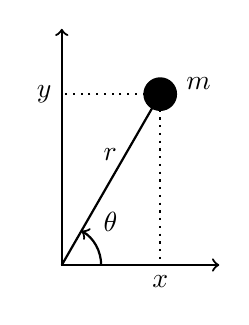
\begin{tikzpicture}[thick]
		\draw [<->,thick] (0,3) |- (2,0);
		\draw [thick] (0,0) -- (1.25, 2.17);
		
		\draw [dotted,thick] (1.25, 2.17) -- (0, 2.17);
		\draw [dotted,thick] (1.25, 2.17) -- (1.25,0);
		
		\draw [fill = black] (1.25,2.17) circle [radius=0.2];
		\draw[->] (0.5,0) arc (0:60:0.5) ;
		
		\node [right] at (1.45,2.3) {$m$};
		\node [right] at (0.4,1.4) {$r$};
		\node [right] at (0.4,0.55) {$\theta$};
		\node [left] at (0, 2.17) {$y$};
		\node [below] at (1.25,0) {$x$};
	\end{tikzpicture}
	\label{fig:examplelagrangian}
	\caption{A free point of mass $m$ in the plane with gravity.}
\end{figure}
			The kinetic and the potential energy for the system are, 
			\begin{equation*}
				T = \frac{1}{2}m(\dot{x}^{2}+\dot{y}^{2}), \quad U = mgy,
			\end{equation*}
			thus taking $\bm{q} = (x;y)\in\mathbb{R}^{2}$ as a vector of generalized coordinates the Lagrangian function is of the form 
			\begin{equation*}
				L = \frac{1}{2}m\transp{\bm{\dot{q}}}\bm{\dot{q}} - mg\transp{\bm{e}}\bm{q},
			\end{equation*}
			where $e_{2}=(0;1)\in\mathbb{R}^{2}$. Nevertheless Cartesian coordinates is not the only possible choice, thus considering \emph{polar} coordinates the following relations hold
			\begin{subequations}
				\begin{align*}
					x &= r\cos{\theta}, & y &= r\sin{\theta}, \\
					\dot{x} &= \dot{r}\cos{\theta} - r\sin{\theta}\dot{\theta}, & \dot{y} &= \dot{r}\sin{\theta}+r\cos{\theta}\dot{\theta},
				\end{align*}
			\end{subequations}
			where $r\in\mathbb{R}_{\geq 0}$ is the radius and $\theta\in[0,2\pi)$ the angular coordinate. Then taking some steps the kinetic and potential energies can be expressed as, 
			\begin{equation*}
				T = \frac{1}{2}m(\dot{r}^{2}+r^{2}\dot{\theta}^{2}), \quad U = mgr\sin{\theta}.
			\end{equation*}
			Thus taking $\widetilde{\bm{q}}:=(\widetilde{q}_{1};\widetilde{q}_{2})=(r;\theta)\in\mathbb{R}^{2}$ as generalized coordinates the Lagrangian is
			\begin{equation}
				L = \frac{1}{2}m(\dot{\widetilde{q}}_{1}^{2}+\widetilde{q}_{1}^{2}\dot{\widetilde{q}}_{2}^{2}) - mg\widetilde{q}_{1}\sin{\widetilde{q}_{2}}.
			\end{equation}
			This simple example shows that the choice of generalized coordinates is not unique but it can be performed according to a criterion of simplicity or utility. As we will see shortly the Lagrangian formulation provides the correct equation of motion despite the chosen reference system. 
		\end{example}
		A very related concept in classical mechanics is the \emph{action} $S\in\mathbb{R}$, this is defined as the integral of the Lagrangian function performed between two instants of time $t_{1},t_{2}\in\mathbb{R}$, i.e.,
		\begin{equation}
			\label{eq:actiondefinition}
			S := \int_{t_{1}}^{t_{2}}L(\bm{q},\dot{\bm{q}},t)\diff t.
		\end{equation}
		Technically speaking the action is a \emph{functional}, i.e., a map that associate to each element of a vector space (usually a space of curves) a scalar. Thus a functional takes curves as input an returns a scalar.
		\begin{remark}
			Notice that $S=S(\bm{q})$ should be thought as a function of $\bm{q}(t)$ over the whole time interval $[t_{1},t_{2}]$. From this point onwards we will use the notation $\bm{q}(\cdot)$ to denote the function $\bm{q}$, while $\bm{q}(t)$ will be denote the \emph{value of function} $\bm{q}$ at the point $t$. Clarified this it is very important to stress that $S$ does not depends on $q(t)$ but from $q(\cdot)$ and it is just a number. Thus for every choice of the ``shape'' of curve $\bm{q}(\cdot)$, the action $S$ assumes a different (scalar) value.
		\end{remark}
		\begin{example}
			Suppose that $\bm{q} = (q_{1};q_{2})\in\mathbb{R}^{2}$, $t_{1} = 0$, $t_{2} = 1$ and $L = q_{1}^{2} + q_{2}^{2}$, thus the action is the following, 
			\begin{equation*}
				S = \int_{0}^{1} q_{1}^2 +q_{2}^{2}\diff t.
			\end{equation*}
			Take now $\bm{q} = (2;t)$, calculating the value for the action results
			\begin{equation*}
				S = \int_{0}^{1} 2^{2} + t^{2}\diff t = \left[4t+\frac{t^{3}}{3}\right]_{0}^{1} = \frac{13}{3}.
			\end{equation*}
		\end{example}
		Similarly as seen in analysis courses you may ask yourself if there exist a curve that minimizes or maximizes the action. The answer has created a new branch of mathematics, i.e., the \emph{calculus of variations}. Calculus of variations concerns the \emph{extremal} of functionals whose domain is an infinite-dimensional space: the space of curves. As we will see shortly the \emph{stationary action principle} simply says that every mechanical system evolves along a curve $\bm{q}(\cdot)$ that is an extremal of the action functional $S$.
		In order to state more formally the stationary action principle, let us consider an initial time $t_{1}$ and an initial configuration associated to it, $\bm{q}_{1} = \bm{q}(t_{1})$, consider also a final time $t_{2}$ and a final configuration $\bm{q}_{2}=\bm{q}(t_{2})$.
		\begin{theorem}[Stationary action]
			\label{th:stationaryaction}
			Motions of mechanical systems from configuration $\bm{q}_{1}$ to configuration $\bm{q}_{2}$, with $t\in[t_{1},t_{2}]$, coincide with extremals curves of the functional in \cref{eq:actiondefinition}. Or equivalently, for small variations of the curve $\bm{q}(\cdot)$ the action $S$ is stationary, i.e.,
			\begin{equation}
				\delta S = 0.
			\end{equation}
		\end{theorem}
		Where $\delta$ denotes a small perturbation of the functional $S$ and sometimes it is also called \emph{variational operator}.
		\begin{example}
			The $\delta$ operator can be successfully applied also to ordinary calculus. Let us consider the function $f(x,y) = \cos(x) + y^2$, then a variation of $f$ results
			\begin{equation*}
				\delta f = \frac{\partial f}{\partial x}\delta x + \frac{\partial f}{\partial y}\delta y = \begin{pmatrix} \cos{x} & y \end{pmatrix}\begin{pmatrix}\delta x \\ \delta y \end{pmatrix}.
			\end{equation*} 
			In this setting stationary points are the ones that satisfies $\delta f = 0$ since for \emph{first order} variation $(\delta x,\delta y)$ the corresponding variation of $f$ is zero. (The surface is locally flat and the variation on $f$ is visible only at the second order). Therefore the stationary points are $(\frac{\pi}{2}+k\pi,0)$ for $k = 1,2,\dots$.
		\end{example}
		Now let us develop the consequences of this principle. Assuming $L$ regular enough is possible to move the $\delta$ operator under the integral,
		\begin{equation}
			\label{eq:actionvariation}
			\delta S = \int_{t_{1}}^{t_{2}}\delta L(\bm{q},\dot{\bm{q}},t) \diff t = \int_{t_{1}}^{t_{2}}\frac{\partial L}{\partial \bm{q}}\delta \bm{q} + \frac{\partial L}{\partial \dot{\bm{q}}}\delta\dot{\bm{q}} \diff t.  
		\end{equation}
		\begin{remark}
			Notice that variations are performed at \emph{fixed time}, therefore the generic variation $\delta L(\bm{q}(t),\bm{\dot{q}}(t),t) = \frac{\partial L}{\partial\bm{q}}\delta \bm{q}+\frac{\partial L}{\partial\bm{\dot{q}}}\delta\bm{\dot{q}}$ and not $\delta L(\bm{q}(t),\bm{\dot{q}}(t),t)\neq\frac{\partial L}{\partial\bm{q}}\delta \bm{q}+\frac{\partial L}{\partial\bm{\dot{q}}}\delta\bm{\dot{q}}+\frac{\partial L}{\partial t}\delta t$. Moreover we must think at the $\dot{\bm{q}}$ variable as independent of $\bm{q}$, since it can be proven that for small variations those quantities are uncorrelated each other.
		\end{remark}
		Now it is useful to consider the following equality that directly follows from integration by part,
		\begin{equation}
			\label{eq:intbypart}
			\frac{\partial L}{\partial\dot{\bm{q}}}\delta\dot{\bm{q}} = \frac{\diff}{\diff t}\left(\frac{\partial L}{\partial\dot{\bm{q}}}\delta \bm{q}\right)-\frac{\diff}{\diff t}\frac{\partial L}{\partial \bm{\dot{q}}}\delta \bm{q},
		\end{equation}
		then substituting \cref{eq:intbypart} into \cref{eq:actionvariation} results,
		\begin{subequations}
			\begin{align}
				\delta S 
				&= \int_{t_{1}}^{t_{2}}\frac{\diff}{\diff t}\left(\frac{\partial L}{\partial\dot{\bm{q}}}\delta \bm{q}\right)-\frac{\diff}{\diff t}\frac{\partial L}{\partial \bm{q}}\delta \bm{q} + \frac{\partial L}{\partial \bm{q}}\delta \bm{q}\diff t \\
				\label{eq:deltaS}
				&= \left[\frac{\partial L}{\partial\dot{\bm{q}}}\delta \bm{q}\right]_{t_{1}}^{t_{2}}+\int_{t_{1}}^{t_{2}}\left(\frac{\partial L}{\partial \bm{q}}-\frac{\diff}{\diff t}\frac{\partial L}{\partial\dot{\bm{q}}}\right)\delta \bm{q}\diff t \\
				&= \int_{t_{1}}^{t_{2}}\left(\frac{\partial L}{\partial \bm{q}}-\frac{\diff}{\diff t}\frac{\partial L}{\partial\dot{\bm{q}}}\right)\delta \bm{q}\diff t = 0
			\end{align}
		\end{subequations}
		\begin{remark}
			In developing passage (\ref{eq:deltaS}) we used $\left[\frac{\partial L}{\partial\dot{\bm{q}}}\delta \bm{q}\right]_{t_{1}}^{t_{2}} = 0$, since variations $\delta\bm{q}(t_{1}) = \delta\bm{q}(t_{2})$ are assumed to be zero because we fixed \emph{a priori} initial and final conditions $\bm{q}_{1}$,$\bm{q}_{2}$. The concept is graphically illustrated in fig. (\ref{fig:variations}), where a set of possible variations is considered but all are vanishing at the endpoints.
		\end{remark}
		\begin{figure}
	\centering
	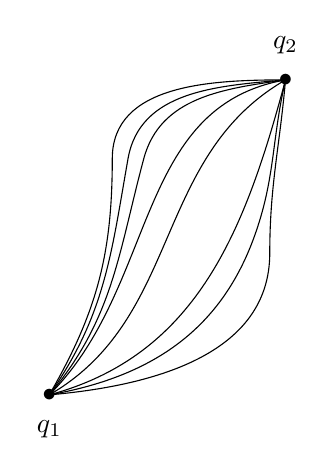
\begin{tikzpicture}
	  \node[label=below:$\bm{q}_1$]  (x1) at (6,0)  {$\bullet$};
	  \node[label=above:$\bm{q}_2$]  (x0) at (9,4)  {$\bullet$};  
	  \draw (x1.center) to [out=5,in=-90]++(2.8,1.8) to[out=90,in=-95](x0.center);
	  \draw (x1.center) to [out=10,in=-110]++(2.6,2) to[out=70,in=-103](x0.center); 
	  \draw (x1.center) to [out=15,in=-105](x0.center);
	  \draw (x1.center) to [out=30,in=-150](x0.center);
	  \draw (x1.center) to [out=45,in=-170](x0.center); 
	  \draw (x1.center) to [out=50,in=-105]++(1.2,3)to [out=75,in=-172](x0.center); 
	  \draw (x1.center) to [out=55,in=-100]++(1.0,3) to[out=80,in=-175](x0.center); 
	  \draw (x1.center) to [out=60,in=-90]++(0.8,3) to[out=90,in=-180] (x0.center);
	\end{tikzpicture}
	\caption{A graphical illustration of the possible variations with fixed endpoints $\bm{q}_{1},\bm{q}_{2}$.}
	\label{fig:variations}  
\end{figure}

		We are now ready to further simplify \cref{eq:deltaS} using the \emph{fundamental lemma of calculus of variations}, which adapted for our purposes states the following:
		\begin{lemma}[Fundamental lemma of calculus of variations]
			\label{lem:foundamentallemma}
			Let $S$ be a \emph{differentiable} (in variational sense) functional, then if
			\begin{equation}
				\int_{t_{1}}^{t_{2}}\left(\frac{\partial L}{\partial \bm{q}}-\frac{\diff}{\diff t}\frac{\partial L}{\partial\dot{\bm{q}}}\right)\delta \bm{q}\diff t = 0,
			\end{equation}
			for any smooth variation $\delta\bm{q}$ with $\delta\bm{q}_{1}=\delta\bm{q}_{2}=0$, then, 
			\begin{equation}
				\label{eq:euleroequations}
				\frac{\diff}{\diff t}\frac{\partial L}{\partial\dot{\bm{q}}}^{\intercal}-\frac{\partial L}{\partial \bm{q}}^{\intercal} = 0.
			\end{equation}
		\end{lemma}	
		The \cref{eq:euleroequations} are called \emph{Euler-Lagrange} equations and they provide the equations of motions for mechanical systems. Roughly speaking \cref{lem:foundamentallemma} states that since the variation $\delta\bm{q}$ is arbitrary, the only way to zeroing the action's variation $\delta S$ is to satisfy Euler-Lagrange equations. Thus we can collect our results in the following theorem.
		\begin{theorem}
			\label{th:minimalaction}
			The curve $q:t\mapsto q(t)$, for $t\in[t_{1},t_{2}]$, is an extremal of the functional $S$ on the space of curves passing through the points $\bm{q}(t_{1}) =\bm{q}_{1}$ and $\bm{q}(t_{2}) = \bm{q}_{2}$, if and only if
			\begin{equation}
				\frac{\diff}{\diff t}\frac{\partial L}{\partial\dot{\bm{q}}}^{\intercal}-\frac{\partial L}{\partial \bm{q}}^{\intercal} = 0.
			\end{equation}
		\end{theorem}
		The key idea of \cref{th:minimalaction} is that a curve $\bm{q}(\cdot)$ in order to be a stationary point for the action $S$, must satisfy the Euler-Lagrange equations, and therefore according to \cref{th:stationaryaction} Euler-Lagrange equations provide the equations of motion for mechanical systems. Notice also that the variational approach is \emph{coordinate free}, meaning that, Euler-Lagrange equations describe the motion regardless the chosen set of coordinates. Indeed the condition for a curve to be an extremal of a functional does not depend on the choice of coordinate systems.
		\begin{example}
			Considering the free mass point in \cref{ex:nonuniquessofq} the equations of motions in the Cartesian coordinates are
			\begin{equation}
				\label{eq:cartesiancoordinates}
				\frac{\diff}{\diff t}\frac{\partial L}{\partial\bm{\dot{q}}}^{\intercal} - \frac{\partial L}{\partial\bm{q}}^{\intercal} = m\ddot{\bm{q}} + mg\bm{e}_{2} = 0,
			\end{equation}
			while in polar coordinates,
			\begin{subequations}
				\begin{align}
					\frac{\diff}{\diff t}\frac{\partial L}{\partial\dot{\widetilde{q}_{1}}} - \frac{\partial L}{\partial\widetilde{q}_{1}} &= m\ddot{\widetilde{q}}_{1} +  mg\sin{\widetilde{q}_{2}}, \\
					\frac{\diff}{\diff t}\frac{\partial L}{\partial\dot{\widetilde{q}_{2}}} - \frac{\partial L}{\partial\widetilde{q}_{2}} &= m\widetilde{q}_{1}^{2}\ddot{\widetilde{q}}_{2} +  2m\widetilde{q}_{1}\dot{\widetilde{q}}_{1}\dot{\widetilde{q}}_{2} + mg\widetilde{q}_{1}\cos{\widetilde{q}_{2}} = 0.
				\end{align}
				\label{eq:polarcoordinates}
			\end{subequations}
			Solutions $q(\cdot)$ and $\widetilde{q}(\cdot)$ respectively solutions of \cref{eq:cartesiancoordinates} and \cref{eq:polarcoordinates} describe the same motion in the plane, just in different coordinate systems.
		\end{example} 
		Nevertheless as presented so far the Euler-Lagrange approach has a big limitation, since $L$ depends only on kinetic and potential energy, we can describe only systems subject to forces that admit a potential function $U$, i.e., \emph{conservative systems}. Luckily the Euler-Lagrange approach can be extended to \emph{nonconservative forces} using the \emph{D'Alembert's principle}, thus \cref{eq:euleroequations} is modified as follows
		\begin{equation}
			\frac{\diff}{\diff t}\frac{\partial L}{\partial\dot{\bm{q}}}^{\intercal}-\frac{\partial L}{\partial \bm{q}}^{\intercal} = \bm{\tau},
		\end{equation}
		where $\bm{\tau}\in\mathbb{R}^{n}$ is a vector of \emph{generalized} non conservative forces.
		
	\section{Mechanical equations of motion}	
		Although Euler-Lagrange equations are very general is often useful to consider an explicit representation for mechanical systems with some special properties. For this purpose we will assume that the kinetic energy $T(\bm{q},\dot{\bm{q}})$ has a very special structure, i.e., is a quadratic form in the generalized velocities $\dot{\bm{q}}$. This is not a very restrictive assumption since every mechanical system with  a finite number of degrees of freedom owns a quadratic kinetic energy. From this simple assumption a lot of interesting properties can be derived; for a good survey see \cite{siciliano2009robotics}. An explicit expression for kinetic energy is
		\begin{equation}
			T(\bm{q},\dot{\bm{q}}) = \frac{1}{2}\sum_{j=1}^{n}\sum_{k=1}^{n}m_{jk}(\bm{q})\dot{q}_{j}\dot{q}_{k} = \frac{1}{2}\dot{\bm{q}}^{\intercal}\bm{M}(\bm{q})\dot{\bm{q}},
		\end{equation}
		where $\bm{M}(\bm{q})\in\mathbb{R}^{n\times n}$ is a symmetric positive definite matrix, usually called \emph{mass matrix}. The entries $m_{jk}(\bm{q})\in\bm{M}(\bm{q})$, for $j,k=1,\dots,n$ are \emph{generalized masses} and \emph{generalized inertias}.
		\begin{remark}
			The matrix $\bm{M}(\bm{q})$ is symmetric since the quadratic form associated to a matrix only depends on symmetric part.
		\end{remark}
		We are now interested in developing an explicit representation for the equations of motion associated to mechanical systems with a \emph{quadratic} kinetic energy. In order to do so we need to perform some tedious calculations. Let us start from Euler-Lagrange equations in \cref{eq:euleroequations}, the term $\frac{\diff}{\diff t}\frac{\partial L}{\partial \dot{q}_{i}}$ appears as
		\begin{equation*}
			\frac{\diff}{\diff t}\frac{\partial L}{\partial \dot{q}_{i}} = \frac{\diff}{\diff t}\frac{\partial T}{\partial \dot{q}_{i}} = \frac{\diff}{\diff t}\frac{\partial}{\partial\dot{q}_{i}}\left(\frac{1}{2}\sum_{j=1}^{n}\sum_{k=1}^{n}m_{jk}(\bm{q})\dot{q}_{j}\dot{q}_{k}\right).
		\end{equation*}
		for $i = 1,\dots,n$. Then exploiting the linearity of summation we can exchange the order between partial derivative and the sum, so that 
		\begin{subequations}
			\label{eq:blekinetic}
			\begin{align}
				\frac{\diff}{\diff t}\frac{\partial L}{\partial \dot{q}_{i}} &= \frac{\diff}{\diff t}\left(\frac{1}{2}\sum_{j=1}^{n}\sum_{k=1}^{n}m_{jk}(\bm{q})\frac{\partial\dot{q}_{j}}{\partial\dot{q}_{i}}\dot{q}_{k}+\frac{1}{2}\sum_{j=1}^{n}\sum_{k=1}^{n}m_{jk}(\bm{q})\dot{q}_{j}\frac{\partial\dot{q}_{k}}{\partial\dot{q}_{i}}\right) \\
				&=\frac{\diff}{\diff t}\left(\frac{1}{2}\sum_{k=1}^{n}m_{ik}(\bm{q})\dot{q}_{k}+\frac{1}{2}\sum_{j=1}^{n}m_{ji}(\bm{q})\dot{q}_{j}\right) = \frac{\diff}{\diff t}\left(\sum_{j=1}^{n}m_{ij}(\bm{q})\dot{q}_{j}\right).
			\end{align}
		\end{subequations}
		In last passage we used the fact that $\frac{\partial\dot{q}_{j}}{\partial\dot{q}_{i}} = 1$ for $i = j$ and $0$ otherwise, and the same holds for $\frac{\partial\dot{q}_{k}}{\partial\dot{q}_{i}}$, moreover we also used the symmetry $m_{ij}(\bm{q})=m_{ji}(\bm{q})$ for $i,j = 1,\dots,n$. Finally deriving with respect to time results, 
		\begin{equation}
			\label{eq:firstparteulerlagrange}
			\frac{\diff}{\diff t}\frac{\partial L}{\partial\dot{q}_{i}} = \sum_{j=1}^{n}m_{ij}(\bm{q})\ddot{q}_{j} + \sum_{j=1}^{n}\sum_{k=1}^{n}\frac{\partial m_{ij}(\bm{q})}{\partial q_{k}}\dot{q}_{k}\dot{q}_{j}.
		\end{equation}
		The obtained expression in \cref{eq:firstparteulerlagrange} is just a part of the Euler-Lagrange equations; considering then the term $\frac{\partial L}{\partial q_{i}}$, for $i=1,\dots,n$, results 
		\begin{equation}
			\label{eq:secondparteulerlagrange}
			\frac{\partial L}{\partial q_{i}} = \frac{1}{2} \sum_{j=1}^{n}\sum_{k=1}^{n}\frac{\partial m_{jk}(\bm{q})}{\partial q_{i}}\dot{q}_{k}\dot{q}_{j} -\frac{\partial U(\bm{q},t)}{\partial q_{i}}.
		\end{equation}
		In order to obtain a more compact representation let us define 
		\begin{equation*}
			g_{i}(\bm{q}) := \frac{\partial U(\bm{q},t)}{\partial q_{i}},
		\end{equation*}
		for $i=1,\dots,n$ and the associate vector $\bm{g}(\bm{q}):=(g_{1}(\bm{q});\dots;g_{n}(\bm{q}))\in\mathbb{R}^{n}$. Combining together \cref{eq:firstparteulerlagrange} and \cref{eq:secondparteulerlagrange}, the overall equations of motion written componentwise result,
		\begin{equation}
			\label{eq:lageqbla}
			\sum_{j=1}^{n}m_{ij}(\bm{q})\ddot{q}_{j} + \sum_{j=1}^{n}\sum_{k=1}^{n}\frac{\partial m_{ij}(\bm{q})}{\partial q_{k}}\dot{q}_{j}\dot{q}_{k} -\frac{1}{2}\sum_{j=1}^{n}\sum_{k=1}^{n}\frac{\partial m_{jk}(\bm{q})}{\partial q_{i}}\dot{q}_{j}\dot{q}_{k}+g_{i}(\bm{q}) = \tau_{i},
		\end{equation}
		for $i=1,\dots,n$. As it is clear from \cref{eq:lageqbla} there is a quadratic term in the generalized velocities $\dot{q}_{j}\dot{q}_{k}$, therefore it is convenient to introduce the symbol $h_{ijk}(\bm{q})\in\mathbb{R}$, with $i,j,k = 1,\dots,n$, defined as
		\begin{equation}
			\label{eq:lagsymbols}
			h_{ijk}(\bm{q}) := \frac{\partial m_{ij}(\bm{q})}{\partial q_{k}}-\frac{1}{2}\frac{\partial m_{jk}(\bm{q})}{\partial q_{i}}. 
		\end{equation}
		Thus substituting \cref{eq:lagsymbols} into \cref{eq:lageqbla} the equations of motion result in the more compact representations
		\begin{equation}
			\label{eq:equationofmotioncomponent}
			\sum_{j=1}^{n}m_{ij}(\bm{q})\ddot{q}_{i} + \sum_{j=1}^{n}\sum_{k=1}^{n}h_{ijk}(\bm{q})\dot{q}_{j}\dot{q}_{k} + g_{i}(\bm{q}) = \tau_{i},
		\end{equation}
		for $i=1,\dots,n$. Now let us analyse \cref{eq:equationofmotioncomponent} to provide a physical interpretation of the different terms:
		\begin{itemize}
			\item The coefficients $m_{ii}(\bm{q})$, with $i =1,\dots,n$, represent the generalized masses associated to the $i$-th degree of freedom.
			\item The coefficients  $m_{ij}(\bm{q})$, with $i,j =1,\dots,n$ but $i\neq j$, represent the \emph{inertia forces} induced by the $j$-th degree of freedom over the $i$-th. 
			\item The quadratic terms $h_{ijj}\dot{q}_{j}^{2}$, with $j = 1,\dots,n$, represent \emph{centrifugal effect} induced on the $i$-th degree of freedom by the $j$-th. Notice that the $i$-th degree of freedom does not induce any centrifugal effect on itself, i.e., $h_{iii}$ = 0.
			\item The terms $h_{ijj}\dot{q}_{j}\dot{q}_{k}$, with $j,k=1,\dots,n$ but $i\neq j$ represents the \emph{Coriolis} effects induced on the degree of freedom $i$-th by velocities of degrees of freedom $j$-th and $k$-th.
			\item The terms $g_{i}(\bm{q})$, with $i=1,\dots,n$, represent the \emph{conservative generalized forces} acting on the $i$-th degree of freedom.
		\end{itemize}
		At this point it is very useful to rewrite the equations of motion (\ref{eq:equationofmotioncomponent}) in a compact matrix notation as follows:
		\begin{equation}
			\bm{M}(\bm{q})\ddot{\bm{q}} + \bm{C}(\bm{q},\dot{\bm{q}})\dot{\bm{q}} + \bm{g}(\bm{q}) = \bm{\tau},
		\end{equation}
		where $\bm{C}(\bm{q},\dot{\bm{q}})$ is a suitable matrix that takes into account the centrifugal and the Coriolis effects. The choice of this matrix is not unique, since it is sufficient that the elements $c_{ij}$ satisfies the relation
		\begin{equation}
			\sum_{j=1}^{n}c_{ij}(\bm{q})\dot{q}_{j} = \sum_{j=1}^{n}\sum_{k=1}^{n}h_{ijk}(\bm{q})\dot{q}_{j}\dot{q}_{k}.
		\end{equation}
		Nevertheless a very common choice is to set the elements $c_{ij}(\bm{q})\in\bm{C}(\bm{q},\dot{\bm{q}})$ as
		\begin{equation}
			\label{eq:coriolismatrixdefinition}
			c_{ij}(\bm{q}) = \sum_{k=1}^{n}c_{ijk}(\bm{q})\dot{q}_{k},
		\end{equation}
		with $i,j=1,\dots,n$. Here the symbol $c_{ijk}(\bm{q})\in\mathbb{R}$ is called \emph{Christoffel symbols of the first type} and it is defined as
		\begin{equation}
			c_{ijk}(\bm{q}) = \frac{1}{2}\left(\frac{\partial m_{ij}(\bm{q})}{\partial q_{k}}+\frac{\partial m_{ik}(\bm{q})}{\partial q_{j}}-\frac{\partial m_{jk}(\bm{q})}{\partial q_{i}}\right).
		\end{equation}
		Notice that thanks to the symmetry of $\bm{M}(\bm{q})$ the following remarkable property of indici exchange holds,
		\begin{equation}
			c_{ijk}(\bm{q}) = c_{ikj}(\bm{q}).
		\end{equation}
		Moreover, if the Coriolis-centrifugal matrix $C(\bm{q},\dot{\bm{q}})$ is chosen according to \cref{eq:coriolismatrixdefinition}, then the following matrix
		\begin{equation}
			\dot{\bm{M}}(\bm{q})-2\bm{C}(\bm{q},\dot{\bm{q}}),
		\end{equation}
		is skew symmetric. This property is sometimes useful to synthesize control algorithms for mechanical systems.
		
	\section{Euler-Lagrange equations with redundant coordinates}
		What we developed until now holds for systems with a \emph{minimum set of coordinates}. Nevertheless for many real systems is quite hard to write directly kinetic and potential energy using a small set of coordinates. A more common approach is to introduce more generalized coordinates than necessary and then add constraints. This fact provides the motivation to investigate the equations of motions for mechanical systems using a non-minimum set of generalized coordinates. For this purpose let us consider that vector $\bm{q}\in\mathbb{R}^{n}$ \emph{does not} represent a minimum set of coordinates. Therefore in order to correctly represent the system we need to impose some constraints. A set of constrain equations can be formally thought as a vectorial function of the form $\bm{\phi}:\mathbb{R}^{n}\times\mathbb{R}\rightarrow\mathbb{R}^{m}$ where $m$ is the number of constrains. The type of constraints equations that we consider are \emph{holomic}, meaning that they depend only on generalized coordinates $\bm{q}$ and possibly time $t$. Holomic constrains can be expressed in the following general form,
		\begin{equation}
			\label{eq:constraintsequations}
			\bm{\phi}(\bm{q},t) = 0.
		\end{equation}
		\begin{remark}
			The total number of degrees of freedom for the system is not $n-m$, unless some regularity for $\bm{\phi}(\bm{q},t)$ is assumed. Technically if $\forall\bm{q}\in\mathbb{R}^{n}$, $\forall t\in\mathbb{R}$ the $\rank{\frac{\partial\bm{\phi}(\bm{q},t)}{\partial \bm{q}}} = m$, then constraints are globally linearly independent each other and the system owns exactly $n-m$ degrees of freedom. Trivially we implicitly assumed that $\bm{\phi}$ is differentiable.
		\end{remark}
		Now our aim is to derive the equations of motions for a constrained mechanical systems described by a Lagrangian function $L(\bm{q},\dot{\bm{q}},t)$ and subject to constrain equation $\bm{\phi}(\bm{q},t)=0$. In order to do so, we can use the technique of Lagrange multipliers on functional spaces. So let us define the \emph{modified action} $\bar{S}\in\mathbb{R}$ as 
		\begin{equation}
			\label{eq:modifiedaction}
			\bar{S} := \int_{t_{1}}^{t_{2}}L(\bm{q},\dot{\bm{q}},t)+\bm{\lambda}^{\intercal}\bm{\phi}(\bm{q},t)\diff t. 
		\end{equation}
		Here $\lambda\in\mathbb{R}^{m}$ is a time dependent vector of \emph{Lagrange multipliers}. The following result is fundamental for our purpose.
		\begin{theorem}[Stationary action for constrained systems]
			Motion of mechanical systems from configuration $\bm{q}_{1}$ to configuration $\bm{q}_{2}$, with $t\in[t_{1}; t_{2}]$, coincide with extremals curves of the functional (\ref{eq:modifiedaction}). Or equivalently, for small variations of the curve $\bm{q}(\cdot)$ the modified action $\bar{S}$ is stationary, i.e.,
			\begin{equation*}
				\delta\bar{S} = 0.
			\end{equation*}
		\end{theorem}
		\begin{remark}
			Notice that we implicitly assumed that initial and final configuration $\bm{q}_{1}$, $\bm{q}_{2}$ are consistent with constrain equations, i.e., $\bm{\phi}(\bm{q}_{1},t_{1}) = \bm{\phi}(\bm{q}_{2},t_{2})= 0$.
		\end{remark}
		Thus we can think to perform variation as done before for systems with a minimal set of coordinates, but there is a difference, since now $\bar{S}$ also depends on the Lagrange multipliers. Therefore the variational operator $\delta$ performs variations on $\bm{q}$, $\bm{\dot{q}}$ and $\bm{\lambda}$. The result is the following,
		\begin{subequations}
			\begin{align}
				\label{eq:variationmodifiedaction}
				\delta\bar{S} &= \int_{t_{1}}^{t_{2}}\delta L(\bm{q},\dot{\bm{q}},t)+\delta\bm{\lambda}^{\intercal}\bm{\phi}(\bm{q},t)+\bm{\lambda}^{\intercal}\delta\bm{\phi}(\bm{q},t)\diff t\\
				&=  \int_{t_{1}}^{t_{2}}\left(\frac{\partial L}{\partial\bm{q}} - \frac{\diff}{\diff t}\frac{\partial L}{\partial\dot{\bm{q}}}+\bm{\lambda}^{\intercal}\frac{\partial\bm{\phi}}{\partial\bm{q}}\right)\delta\bm{q} + +\delta\bm{\lambda}^{\intercal}\bm{\phi}(\bm{q},t)\diff t + \left[\frac{\partial L}{\partial\dot{\bm{q}}}\delta\bm{q} \right]_{t_{1}}^{t_{2}}\\
				&=\int_{t_{1}}^{t_{2}}
				\begin{bmatrix}
					\frac{\partial L}{\partial\bm{q}} - \frac{\diff}{\diff t}\frac{\partial L}{\partial\dot{\bm{q}}} + \bm{\lambda}^{\intercal}\frac{\partial\bm{\phi}}{\partial\bm{q}} & \bm{\phi}^{\intercal}
				\end{bmatrix}
				\begin{bmatrix}
					\delta\bm{q} \\
					\delta\bm{\lambda}
				\end{bmatrix} \diff t = 0,
			\end{align}
		\end{subequations} 
		again we used that endpoints variations $\delta\bm{q}_{1} = \delta\bm{q}_{2} = 0$. Finally applying the fundamental lemma of calculus of variations \cref{eq:variationmodifiedaction}, results
		\begin{subequations}
			\label{eq:mechanicalDAE}
			\begin{align}
				\frac{\diff}{\diff t}\frac{\partial L}{\partial\dot{\bm{q}}}^{\intercal}-\frac{\partial L}{\partial \bm{q}}^{\intercal} &= \frac{\partial\bm{\phi}}{\partial\bm{q}}^{\intercal}\bm{\lambda}, \\
				\bm{\phi}(\bm{q},t) &= 0.
			\end{align}
		\end{subequations}
		The equations (\ref{eq:mechanicalDAE}) describe the motion of a mechanical system subject to holomic constraints. Note that the term $\frac{\partial\bm{\phi}}{\partial\bm{q}}^{\intercal}\bm{\lambda}$ plays the role of a constrain generalized force which pushes the system to satisfy the constraints $\bm{\phi}(\bm{q},t) = 0$. Unfortunately problem in \cref{eq:mechanicalDAE} is completely different from the one in \cref{eq:euleroequations}, since it is a mixture of \emph{differential} and \emph{algebraic} equations, formally a \emph{Differential Algebraic Equation} (DAE). Moreover, apparently \cref{eq:mechanicalDAE}, does not provide any way to determine the value of the Lagrange multipliers. Similarly in presence of external non-conservative generalized forces the equation of motions for a constrained mechanical system are modified as follows,
		\begin{subequations}
			\begin{align}
				\frac{\diff}{\diff t}\frac{\partial L}{\partial\dot{\bm{q}}}^{\intercal}-\frac{\partial L}{\partial \bm{q}}^{\intercal} &= \frac{\partial\bm{\phi}}{\partial\bm{q}}^{\intercal}\bm{\lambda}+\bm{\tau},\\
				\bm{\phi}(\bm{q},t) &= 0,
			\end{align}
		\end{subequations}
		again with $\tau\in\mathbb{R}^{n}$ a vector of generalized non-conservative forces.
		\begin{example}
			\label{ex:pendulum1}
			Let us consider a simple mechanical example, the pendulum, see \cref{fig:pendulum}. 
			\begin{figure}
	\centering
	\label{fig:pendulum}
	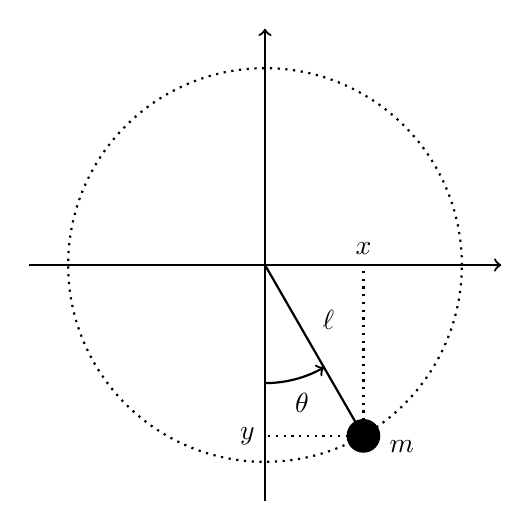
\begin{tikzpicture}[thick]
		\draw [<->,thick] (0,3) |- (3,0);
		\draw [-] (0,-3) |- (-3,0);
		\draw [thick] (0,0) -- (1.25, -2.17);
		
		\draw [dotted,thick] (1.25, -2.17) -- (0, -2.17);
		\draw [dotted,thick] (1.25, -2.17) -- (1.25,0);
		
		\draw [dotted,color=black] circle(2.5);
		\draw [fill = black] (1.25,-2.17) circle [radius=0.2];
		\draw[->] (0,-1.5) arc (-90:-60:1.5) ;
		
		\node [right] at (1.45,-2.3) {$m$};
		\node [right] at (0.6,-0.7) {$\ell$};
		\node [right] at (0.25,-1.75) {$\theta$};
		\node [left] at (0, -2.17) {$y$};
		\node [above] at (1.25,0) {$x$};
	\end{tikzpicture}
	\caption{A simple pendulum.}
\end{figure}

			Pendulum own one-degree of freedom and taking the angular coordinate $\theta\in[0,2\pi)$ as generalized coordinate, the following relationships with $(x,y)\in\mathbb{R}^{2}$ hold, 
			\begin{equation*}
					x = \ell\sin{\theta}, \quad y = -\ell\cos{\theta}.
			\end{equation*}
			Thus kinetic and potential energy can be expressed as, 
			\begin{equation*}
				T(\theta) = \frac{1}{2}m(\dot{x}^{2}+\dot{y}^{2}) = \frac{1}{2}m\ell^{2}\dot{\theta}^{2},\quad U(\theta) = gmy = -gm\ell\cos{\theta}, 
			\end{equation*}
			while the Lagrangian for the system results, 
			\begin{equation*}
				L = \frac{1}{2}m\ell^{2}\dot{\theta}^{2} + gm\ell\cos{\theta}.
			\end{equation*}
			Using the Euler-Lagrange equations in \cref{eq:euleroequations} yields to
			\begin{equation*}
				\frac{\diff}{\diff t}\frac{\partial L}{\partial\dot{\theta}}-\frac{\partial L}{\partial\theta} = m\ell^{2}\ddot{\theta} + mg\ell\sin{\theta} = 0,
			\end{equation*}
			which can be simplified to
			\begin{equation*}
				\ddot{\theta} = -\frac{g}{\ell}\sin{\theta}.
			\end{equation*}
			Now suppose we want to describe the pendulum using a set of redundant coordinates, e.g., \emph{natural coordinates}. For this aim let us define the generalized coordinate $\bm{q} = (x;y)\in\mathbb{R}^{2}$. The associated Lagrangian function takes the form, 
			\begin{equation*}
				L = \frac{1}{2}m\transp{\dot{\bm{q}}}\bm{\dot{q}} - mg\transp{\bm{e}}_{2}\bm{q},
			\end{equation*}
			where $\bm{e}_{2}\in\mathbb{R}^{2}$ is the second vector of the natural basis, roughly speaking the vector $\bm{e}_{2} = (0;1)\in\mathbb{R}^{2}$. Obviously now we need to introduce some constraint equation in order to force mass $m$ to slide over the circle, i.e., 
			\begin{equation*}
				\phi(\bm{q}) = x^{2}+y^{2} - \ell^{2} = \transp{\bm{q}}\bm{q}-\ell^{2} = 0.
			\end{equation*}
			Using then \cref{eq:mechanicalDAE} the resultant system of equations is the following, 
			\begin{subequations}
				\begin{align*}
					m\ddot{\bm{q}} + mg\bm{e}_{2} &= 2\bm{q}\lambda, \\
					\transp{\bm{q}}\bm{q}-\ell^{2} &= 0.
				\end{align*}
			\end{subequations}
		\end{example}
		
	\section{Resolution of Mechanical DAEs}
		As well pointed out in \cite{petzold1982differential} both from theoretical point of view that the numerical, DAEs are much more challenging than ordinary differential equations (ODEs). Some DAEs can be solved using numerical methods for stiff systems but others cannot and they are very sensitive to the step size and this may cause large errors in the solution and numerical instability. For DAEs coming from constrained mechanical systems a fairly general form is the following, 
		\begin{subequations}
		\label{eq:generalformequationofmotion}
			\begin{align}
				\bm{M}(\bm{q})\ddot{\bm{q}} -\frac{\partial\bm{\phi}}{\partial\bm{q}}^{\intercal}\lambda &= \bm{n}(\bm{q},\dot{\bm{q}},t),\\
				\bm{\phi}(\bm{q},t) &= 0
			\end{align}
		\end{subequations}
		where the term $\bm{n}(\bm{q},\dot{\bm{q}},t)\in\mathbb{R}^{n}$ collects all the contributions coming from Coriolis and centrifugal effects, conservative and non-conservative forces, e.g., it may be definite as follows,
		\begin{equation*}
			\bm{n}(\bm{q},\dot{\bm{q}},t) = \bm{\tau}-\bm{C}(\bm{q},\dot{\bm{q}})\dot{\bm{q}}-\bm{g}(\bm{q}).
		\end{equation*}
		It is well known that the equations of motion for a mechanical system are a system of second order (possibly) non-linear differential equations. However for clarity and for sake of generality  it is useful to consider a \emph{first order representation}. For this purpose let us define $\bm{p}\in\mathbb{R}^{n}$ as \emph{generalized velocities}, i.e.,
		\begin{equation}
			\label{eq:firstordersubstitution}
			\bm{p} := \dot{\bm{q}}.
		\end{equation}
		Thus substituting \cref{eq:firstordersubstitution} into \cref{eq:generalformequationofmotion} results, 
		\begin{subequations}
		\label{eq:generalequationofmotionfirstorder}
			\begin{align}
				\dot{\bm{q}} &= \bm{p}, \\
				\bm{M}(\bm{q})\dot{\bm{p}} -\frac{\partial\bm{\phi}}{\partial\bm{q}}^{\intercal}\bm{\lambda} &= \bm{n}(\bm{q},\bm{p},t),\\
				\bm{\phi}(\bm{q},t) &= 0.
			\end{align}
		\end{subequations}
		Notice that the vector $(\bm{q};\bm{p})\in\mathbb{R}^{2n}$ represents the \emph{state} of a mechanical system, namely the pair \emph{generalized position} and \emph{generalized velocity}.
		
		Now a good question is how to solve the problem in \cref{eq:generalequationofmotionfirstorder}, the issue is certainly how to determine the value for the Lagrange multiplier $\bm{\lambda}$. One possible approach is to transform the problem into a system of pure differential equations. In order to do so we need to differentiate the constraint $\bm{\phi}(\bm{q},t)$, this yields to
		\begin{equation}
			\label{eq:diffconstraint}
			\frac{\diff\bm{\phi}}{\diff t} = \frac{\partial\bm{\phi}}{\partial\bm{q}}\bm{p}+\frac{\partial\bm{\phi}}{\partial t}=0.
		\end{equation}
		Notice that when constraint does not depend on time \cref{eq:diffconstraint} expresses the intuitive idea that generalized velocity $\bm{p}$ must be orthogonal to constraint's gradient. This provide also the opportunity to notice that constraint $\bm{\phi}(\bm{q},t)$ imposes relationships also at the velocity and acceleration level, e.g., \cref{eq:diffconstraint} restricts the set of feasible velocities. The constraints can we can obtain differentiating the constraint are somehow called \emph{hidden constraints}. Finally notice that \cref{eq:diffconstraint} is still algebraic in the $\bm{p}$ coordinate, thus in order to obtain a differential relationship let us differentiate again,
		\begin{equation}
			\label{eq:ddiffconstraint}
			\frac{\diff^2\bm{\phi}(\bm{q},t)}{\diff t^2} = \frac{\diff}{\diff t}\frac{\partial\bm{\phi}}{\partial\bm{q}}\bm{p} +\frac{\partial\bm{\phi}}{\partial\bm{q}}\bm{\dot{p}}+\frac{\partial^2\bm{\phi}}{\partial t^2}=0.
		\end{equation}
		Notice that now \cref{eq:ddiffconstraint} does not impose any algebraic constraint on the state of the mechanical system $(\bm{q};\bm{p})$ . Thus substituting the constraint $\bm{\phi}(\bm{q},t) = 0$ with the one in \cref{eq:ddiffconstraint} results the following modified problem,
		\begin{subequations}
		\label{eq:generalequationofmotionfirstorderdiffconstraint}
			\begin{align}
				\dot{\bm{q}} &= \bm{p}, \\
				\bm{M}(\bm{q})\dot{\bm{p}} -\frac{\partial\bm{\phi}}{\partial\bm{q}}^{\intercal}\bm{\lambda} &= \bm{n}(\bm{q},\bm{p},t),\\
				-\frac{\partial\bm{\phi}}{\partial\bm{q}}\bm{\dot{p}} &= \frac{\diff}{\diff t}\frac{\partial\bm{\phi}}{\partial\bm{q}}\bm{p} +\frac{\partial^2\bm{\phi}}{\partial t^2} := \bm{m}(\bm{q},\bm{p},t).
			\end{align}
		\end{subequations}
		Here to simplify the notation we introduced the symbol $\bm{m}(\bm{q},\bm{p},t)\in\mathbb{R}^{m}$. However even if the idea of differentiating the constraint seem good, the problem in \cref{eq:mechanicalDAE} and the one in \cref{eq:generalequationofmotionfirstorderdiffconstraint} are \emph{not equivalent}. This difference produces the so called \emph{drift effect} that will be investigated in next section. At the moment let us ignore this complication and continue on the taken path. System of equations in \cref{eq:generalequationofmotionfirstorderdiffconstraint} can be also written in compact matrix notation as,
		\begin{equation}
			\label{eq:numericalscheme}
			\begin{bmatrix}
				\bm{I} 	&	0		&	0 \\
				0	& 	\bm{M}(\bm{q}) 	&	-\frac{\partial\bm{\phi}}{\partial\bm{q}}^{\intercal} \\
				0 	& -\frac{\partial\bm{\phi}}{\partial\bm{q}} & 0\\
			\end{bmatrix}
			\begin{bmatrix}
				\dot{\bm{q}}\\
				\dot{\bm{p}}\\
				\bm{\lambda}
			\end{bmatrix}
			= 
			\begin{bmatrix}
				\bm{p} \\
				\bm{n}(\bm{q},\bm{p},t) \\
				\bm{m}(\bm{q},\bm{p},t)
			\end{bmatrix}.
		\end{equation}
		Now it's easy to see that if the matrix on the left hand side of \cref{eq:numericalscheme} is invertible, then we can express the system in explicit form and use this representation to perform numerical simulations. 		
		It easy to see that the matrix is invertible if and only if the sub-block,
		\begin{equation*}
			\begin{bmatrix}
				\bm{M}(\bm{q}) & -\frac{\partial\bm{\phi}}{\partial\bm{q}}^{\intercal} \\
				-\frac{\partial\bm{\phi}}{\partial\bm{q}} & 0
			\end{bmatrix}\in\mathbb{R}^{(n+m)\times(n+m)},
		\end{equation*}
		is non-singular (full rank). In order to prove this we can use the rank additivity formula which states the following, 
		\begin{equation*}
		 	\rank{\begin{bmatrix}
		 		\bm{M}(\bm{q}) & -\frac{\partial\bm{\phi}}{\partial\bm{q}}^{\intercal} \\
		 		-\frac{\partial\bm{\phi}}{\partial\bm{q}} & 0
		 	\end{bmatrix}} 
		 	= \rank{\bm{M}(\bm{q})} + \rank{\left( \frac{\partial\bm{\phi}}{\partial\bm{q}}\bm{M}(\bm{q})^{-1}\frac{\partial\bm{\phi}}{\partial\bm{q}}^{\intercal}\right)}.
		\end{equation*}
		First recall that matrix $\bm{M}(\bm{q})$ is positive definite (so also non-singular), then $\forall\bm{q}\in\mathbb{R}^{n}, \rank{\bm{M}(\bm{q})} = n$. Thus what is missing is the condition 
		\begin{equation}
			\label{eq:compression}
			\rank{\left( \frac{\partial\bm{\phi}}{\partial\bm{q}}\bm{M}(\bm{q})^{-1}\frac{\partial\bm{\phi}}{\partial\bm{q}}^{\intercal}\right)} = m,
		\end{equation}
		which is not generally true. Fortunately assuming the constraints (locally) linearly independent each other, i.e., $\forall\bm{q}\in\mathbb{R}^{n},\forall t$
		\begin{equation}
			\label{eq:independentcondition}
			\rank{\left(\frac{\partial\bm{\phi}}{\partial\bm{q}}\right)} = m, 
		\end{equation}
		\cref{eq:compression} holds, matrix in \cref{eq:numericalscheme} is invertible and the overall system can be expressed in \emph{explicit first order form} as follows,
		\begin{equation*}
			\begin{bmatrix}
				\dot{\bm{q}}\\
				\dot{\bm{p}}\\
				\bm{\lambda}
			\end{bmatrix}
			= 
			\begin{bmatrix}
				\bm{I} 	&	0		&	0 \\
				0	& 	\bm{M}(\bm{q}) 	&	-\frac{\partial\bm{\phi}}{\partial\bm{q}}^{\intercal} \\
				0 	& -\frac{\partial\bm{\phi}}{\partial\bm{q}} & 0\\
			\end{bmatrix}^{-1}
			\begin{bmatrix}
				\bm{p} \\
				\bm{n}(\bm{q},\bm{p},t) \\
				\bm{m}(\bm{q},\bm{p},t)
			\end{bmatrix}.
		\end{equation*}
		An explicit expression for the inverse matrix above can be obtained through tedious calculations and it is shown in \cref{subsec:matrixinverse}. However regardless the specific expression of the solution we want stress a very important point; differentiating the constraint we were able to find an explicit expression for the Lagrange multipliers. For this purpose we differentiated twice and we obtained \cref{eq:ddiffconstraint}. Then isolating the acceleration $\bm{\dot{p}}$ from \cref{eq:generalequationofmotionfirstorder} results,
		\begin{equation}
			\label{eq:genvelo}
			\dot{\bm{p}} = \bm{M}(\bm{q})\frac{\partial\bm{\phi}}{\partial\bm{q}}^{\intercal}\bm{\lambda}+\bm{M}(\bm{q})^{-1}\bm{n}(\bm{q},\bm{p},t) = 0.	
		\end{equation}
		Thus substituting \cref{eq:genvelo} into \cref{eq:ddiffconstraint} results,
		\begin{equation}
			\frac{\diff}{\diff t}\frac{\partial\bm{\phi}}{\partial\bm{q}}\bm{p} + \frac{\partial\bm{\phi}}{\partial\bm{q}}\bm{M}(\bm{q})^{-1}\frac{\partial\bm{\phi}}{\partial\bm{q}}^{\intercal}\bm{\lambda}+\frac{\partial\bm{\phi}}{\partial\bm{q}}\bm{M}(\bm{q})^{-1}\bm{n}(\bm{q},\bm{p},t)+\frac{\partial^{2}\bm{\phi}}{\partial t^{2}}.
		\end{equation}
		Here we recognize the nonsingular matrix in \cref{eq:compression}, therefore an explicit expression for the Lagrange multipliers is the following, 
		\begin{equation*}
			\bm{\lambda} = -\left(\frac{\partial\bm{\phi}}{\partial\bm{q}}\bm{M}(\bm{q})^{-1}\frac{\partial\bm{\phi}}{\partial\bm{q}}^{\intercal}\right)^{-1}\left(\frac{\diff}{\diff t}\frac{\partial\bm{\phi}}{\partial\bm{q}}\bm{p}+\frac{\partial\bm{\phi}}{\partial\bm{q}}\bm{M}(\bm{q})^{-1}\bm{n}(\bm{q},\bm{p},t)+\frac{\partial^{2}\bm{\phi}}{\partial t^{2}}\right). 
		\end{equation*}
		Technically Mechanical systems subject to holonomic constraints are systems of differential-algebraic equations (DAEs) of \emph{differential index} 3. The differential index is one plus the number of differentiations of the constraint that are needed in order to be able to eliminate the Lagrange multipliers. Otherwise, equivalently, the number of times that we need to differentiate the constraint in order to obtain a differential equation also for the Lagrange multiplier. 
		
	\section{The drift effect}
		In this section we want investigate the effects of the differentiating process done to transform problem in \cref{eq:generalequationofmotionfirstorder} into problem \cref{eq:generalequationofmotionfirstorderdiffconstraint}. Unfortunately this method is \emph{not} priceless, indeed formally we substitute an algebraic constraint with its second derivative w.r.t time. To better understand the consequences let us consider a fictitious constraint $\widetilde{\bm{\phi}}(\bm{q},t)$ of the form, 
		\begin{equation}
			\widetilde{\bm{\phi}}(\bm{q},t) := \bm{\phi}(\bm{q},t)+\bm{a}_0 + \bm{a}_{1}t.
		\end{equation}
		It is easy to see that consider a mechanical system subject to constraint $\phi(\bm{q},t)$ or $\widetilde{\bm{\phi}}(\bm{q},t)$ differentiating twice is exactly the same, i.e.,
		\begin{equation}
			\frac{\diff^2\bm{\phi}}{\diff t^2} = \frac{\diff^2\widetilde{\bm{\phi}}}{\diff t^2}.
		\end{equation}    
		This fact produces the \emph{drift effect}, i.e., the original constraint $\bm{\phi}(\bm{q},t)$ is violated with an error growing with time. This error grows in the best case linearly, but it can be faster due to \emph{numerical} errors. The reason of this behaviour is the term $\bm{a}_{1}t$ which does not have any effect in the formulation (\ref{eq:generalequationofmotionfirstorderdiffconstraint}). Note also that this is not an undesired effect coming from not enough precision of the numerical scheme, but it is intrinsic effect due to substitution of the constraint $\bm{\phi}$ with its second derivative w.r.t time. A simple solution to this undesired effect is the Baumgarte's stabilization that we will discuss in the next section.
		\begin{example}
			\label{ex:pendulum2}
			Continuing \cref{ex:pendulum1} we provide a first order representation for the pendulum; setting $\bm{p} = \dot{\bm{q}}$ results, 
			\begin{subequations}
				\begin{align*}
					\bm{p} = \dot{\bm{q}},\\
					m\dot{\bm{p}} + mg\bm{e}_{2} = 2\bm{q}\lambda,\\
					\transp{\bm{q}}\bm{q} - \ell^{2} = 0.
				\end{align*}
			\end{subequations}
			Then in order to eliminate the Lagrange multiplier let us differentiate the constraint, 
			\begin{equation*}
				\frac{\diff\phi}{\diff t} = 2\transp{\bm{q}}\bm{p} = 0.
			\end{equation*}
			Notice that as expected velocity $\bm{p}$ and position $\bm{q}$ are orthogonal each other. Differentiating again we obtain 
			\begin{equation*}
				\frac{\diff^{2}\phi}{\diff t^2} = 2\transp{\dot{\bm{q}}}\bm{p} + 2\transp{\bm{q}}\dot{\bm{p}} = 2\transp{\bm{p}}\bm{p} + 2\transp{\bm{q}}\dot{\bm{p}} = 0.
			\end{equation*}
			Now we can write the problem in shape of \cref{eq:numericalscheme}, 
			\begin{equation}
				\label{eq:numericalschemependulum}
				\begin{bmatrix}
					\bm{I}_{2} 	& 0 & 0 \\
					0 			& m\bm{I}_{2} & -2\bm{q} \\ 
					0 			& -2\transp{\bm{q}}  & 0
				\end{bmatrix}
				\begin{bmatrix}
					\dot{\bm{q}} \\
					\dot{\bm{p}} \\
					\lambda
				\end{bmatrix}
				= 
				\begin{bmatrix}
					\bm{p} \\
					-mg\bm{e}_{2}\\
					2\transp{\bm{p}}\bm{p}
				\end{bmatrix},
			\end{equation}
		\end{example}
		where $\bm{I}_{2}\in\mathbb{R}^{2\times 2}$ is the identity matrix of dimension 2. The explicit value for the Lagrange multipliers is the following
		\begin{equation}
			\label{eq:explicitlambdapendulum}
			\lambda = -\frac{m}{2\bm{q}^{\intercal}\bm{q}}\left(\bm{p}^{\intercal}\bm{p}-g\bm{q}^{\intercal}\bm{e}_{2}\right) = -\frac{m}{2\ell^{2}}\left(\bm{p}^{\intercal}\bm{p}-gq_{2}\right). 
		\end{equation}
		To better appreciate the drift effect we can simulate \cref{eq:numericalschemependulum} using an ode solver. The results are showed in \cref{fig:trackingerrosr}.
		\begin{figure}[htbp]
			\centering
			\begin{tikzpicture}
				\begin{axis}
					[xmin=-5,xmax=5,ymin=-7.5,ymax=2.5, ytick={-7.5,-5,-2.5,0,2.5,5},grid=both,width=10cm,height=10cm]
					\draw (axis cs:0,0) circle [black, radius=2.5];
					\addplot[dotted,samples=10,color=red]table[x=x1,y=y1]{data/nstab.txt};
				\end{axis}
			\end{tikzpicture}
			\caption{Pendulum simulation with drift effect.}
			\label{fig:trackingerrosr}
		\end{figure}
		Simulation has been performed for $50$ seconds with the following parameters, $g = 9.81$, $m=2$, $\ell=2.5$ and initial conditions $\bm{q}_{0} = (0.86; 2.35)\in\mathbb{R}^{2}$, $\dot{\bm{q}}_{0} = \bm{p}_{0} = (0,0)\in\mathbb{R}^{2}$ and $\lambda_{0} = 3.69$, which are all consistent with the constraint and with \cref{eq:explicitlambdapendulum}.
		
	\section{Baumgarte's stabilization}
		A very popular way to stabilize the constraint $\bm{\phi}(\bm{q},t)=0$ and thus avoid the drift effect is using Baumgarte's stabilization, see \cite{baumgarte1972stabilization}. This idea is well presented with other techniques in the survey paper \cite{ascher1995stabilization}. The key idea is to substitute the constraint with a \emph{differential equation} that \emph{asymptotically} satisfies $\bm{\phi}(\bm{q},t)=0$. Obviously this technique is effective only if you are interested in the \emph{long term} behaviour, since during transients the constraint may be violated. Since constrained mechanical systems require to differentiations to eliminate the Lagrange multipliers, we consider a linear second order stable differential equation of the form, 
		\begin{equation}
			\label{eq:secondordersystem}
			\frac{\diff^2 z(t)}{\diff t^2} + 2\xi\omega_{\textnormal{n}}\frac{\diff z(t)}{\diff t} + \omega_{\textnormal{n}}^2z(t) = 0,
		\end{equation}  
		where $z(t)\in\mathbb{R}$. In this form we recognize the well known equation for second order linear mechanical or electrical systems, such as the \emph{RLC circuit} or the \emph{mass spring damper}. In these framework $\xi\in\mathbb{R}_{>0}$ is the \emph{damping ratio} and $\omega_{\textnormal{n}}\in\mathbb{R}_{>0}$ is the \emph{natural frequency}. Depending on the value of $\xi$ different cases can arise:
		\begin{itemize}
			\item $0<\xi<1$: solution $z$ is \emph{underdamped},
			\item $\xi=1$: solution $z$ is \emph{critically damped},
			\item $\xi>1$: solution $z$ is \emph{overdamped}.
		\end{itemize}
		The general form for the solution is the following
		\begin{equation*}
			z(t) = k_{1}e^{\left(-\xi+\sqrt{\xi^2-1}\right)\omega_{\textnormal{n}}t} + k_{2}e^{\left(-\xi-\sqrt{\xi^2-1}\right)\omega_{\textnormal{n}}t}, 
		\end{equation*}
		where $k_{1},k_{2}\in\mathbb{R}$ are constants determined by the initial conditions $z_{0} = z(t=0)$ and $\dot{z}_{0} = \dot{z}(t=0)$. Solutions for the different cases can be arranged in different ways, here we show some of them. For a deeper treatment see for example \cite{rao1995mechanical}. Let us start from the underdamped case; solution takes the form
		\begin{equation}
			\label{eq:underdamped}
			z(t) = c_ {1}e^{-\xi\omega_{\textnormal{n}}t}\cos\left({\sqrt{1-\xi^2}\omega_{\textnormal{n}}t-c_{2}}\right),
		\end{equation}
		where constants $c_{1},c_{2}\in\mathbb{R}$ are given by, 
		\begin{subequations}
			\begin{align*}
				c_{1} &= \frac{\sqrt{z_{0}^2\omega_{\textnormal{n}}^2+\dot{z}_{0}^2+2z_{0}\dot{z}_{0}\xi\omega_{\textnormal{n}}}}{\sqrt{1-\xi^2}\omega_{\textnormal{n}}}\\
				c_{2} &= \tan^{-1}\left(\frac{\dot{z}_{0}+\xi\omega_{\textnormal{n}}z_{0}}{x_ {0}\omega_{\textnormal{n}}\sqrt{1-\xi^2}}\right).
			\end{align*}
		\end{subequations}
		As we can observe in \cref{eq:underdamped} solution is a cosine function modulated by a decreasing exponential function. For the critically damped case a linear term appears and the solution takes the form, 
		\begin{equation}
			\label{eq:criticallydamped}
			z(t) = (c_{1}+c_{2}t)e^{-\omega_{\textnormal{n}}t},
		\end{equation}
		where $c_{1},c_{2}\in\mathbb{R}$ are given by $c_{1} = z_{0}$ and $c_{2} = \dot{z}_{0}+\omega_{\textnormal{n}}z_{0}$. Finally for the overdamped case the solution takes the form
		\begin{equation}
			\label{eq:overdamped}
			z(t) = c_{1}e^{\left(-\xi+\sqrt{\xi^2-1}\right)\omega_{\textnormal{n}}t} + c_{2}e^{\left(-\xi-\sqrt{\xi^2-1}\right)\omega_{\textnormal{n}}t}, 
		\end{equation}
		with constants, 
		\begin{subequations}
			\begin{align*}
				c_{1} &= \frac{x_{0}\omega_{\textnormal{n}}\left(\xi+\sqrt{\xi^2-1}\right)+\dot{x}_{0}}{2\omega_{\textnormal{n}}\sqrt{\xi^2-1}},\\
				c_{2} &= \frac{-x_{0}\omega_{\textnormal{n}}\left(\xi-\sqrt{\xi^2-1}\right)-\dot{x}_{0}}{2\omega_{\textnormal{n}}\sqrt{\xi^2-1}}.
			\end{align*}
		\end{subequations}
		However, regardless of the specific form of the solution, all the three cases satisfy a \emph{global exponential stability} property, i.e., $\forall(z_{0},\dot{z}_{0})\in\mathbb{R}\times\mathbb{R}$ the solution $z(t,z_{0},\dot{z}_{0})$ satisfies
		\begin{equation*}
			\lim_{t\rightarrow\infty} z(t,z_{0},\dot{z}_{0}) = 0.
		\end{equation*}
		The notation $z(t,z_{0},\dot{z}_{0})$ is just to stress that the solution depends on time but also from initial conditions $(z_{0},\dot{z}_{0})$. This consideration suggests to substitute the constraint $\bm{\phi}(\bm{q},t)$ with an ODE of the form (\ref{eq:secondordersystem}). In this way, despite the initial conditions, the solution will asymptotically satisfies $\bm{\phi}(\bm{q},t)=0$. Thus the explicit \emph{Baumgarte's stabilization} for DAEs of index three takes the form,	
		\begin{equation*}
			\frac{\diff^2\bm{\phi}}{\diff t^2} + 2\xi\omega_{\textnormal{n}}\frac{\diff\bm{\phi}}{\diff t} + \omega_{\textnormal{n}}^2\bm{\phi} = 0.
		\end{equation*}
		Computing explicitly the terms for mechanical systems the stabilization results,
		\begin{equation}
			\frac{\diff}{\diff t}\frac{\partial\bm{\phi}}{\partial\bm{q}}\dot{\bm{q}}+\frac{\partial\bm{\phi}}{\partial\bm{q}}\ddot{\bm{q}}+\frac{\partial^{2}\bm{\phi}}{\partial t^2} + 2\xi\omega_{\textnormal{n}}\frac{\partial\phi}{\partial\bm{q}}\dot{\bm{q}} + 2\xi\omega_{\textnormal{n}}\frac{\partial\bm{\phi}}{\partial t}+\omega_{\textnormal{n}}^2\bm{\phi} = 0.
		\end{equation}
		which can be re-arranged in the following form
		\begin{equation}
			\label{eq:baumstability}
			-\frac{\partial\bm{\phi}}{\partial\bm{q}}\dot{\bm{p}} = \frac{\diff}{\diff t}\frac{\partial\bm{\phi}}{\partial\bm{q}}\bm{p}+\frac{\partial^{2}\bm{\phi}}{\partial t^2} + 2\xi\omega_{\textnormal{n}}\frac{\partial\phi}{\partial\bm{q}}\bm{p} + 2\xi\omega_{\textnormal{n}}\frac{\partial\bm{\phi}}{\partial t}+\omega_{\textnormal{n}}^2\bm{\phi} :=\bm{m}(\bm{q},\bm{p},t).
		\end{equation}
		Now \cref{eq:baumstability} can be easy implemented without any modification in \cref{eq:numericalscheme}; indeed it is sufficient to redefine $\bm{m}(\bm{q},\bm{p},t)$ as in \cref{eq:baumstability}. However a question is still open, how can we tune the parameters $\omega_{\textnormal{n}}$ and $\xi$?. Unfortunately there is not general rule, but it is useful to notice that the velocity of convergence to zero of the solution depends on both$\xi$ and $\omega_{\textnormal{n}}$. Therefore it is a good idea to select them in order to obtain an high decay rate compatibly with the \emph{numerical stability}. This means that the dynamics associated to the constraint $\bm{\phi}(\bm{q},t)$ cannot be too fast compared to other ones, otherwise the system could be very hard (stiff) to simulate numerically. Indeed systems where two or more very different time scales are involved are usually called \emph{stiff problems} or \emph{stiff systems}. These may cause some numerical problems, since stiff equations require an integration step extremely small and are numerically unstable. In general it is hard to provide a unique definition of stiffness, but the main idea is that the differential equations includes some terms that can lead to rapid variation in the solution.
		\begin{example}
			Continuing \cref{ex:pendulum2} we want use the Baumgarte's technique to stabilize the pendulum. Therefore the idea is to substitute the constraint
			\begin{equation*}
				2\bm{p}^{\intercal}\bm{p}+2\bm{q}\dot{\bm{p}} = 0
			\end{equation*}
			with
			\begin{equation*}
				-2\transp{\bm{q}}\dot{\bm{p}} = 2\transp{\bm{p}}\bm{p} + 4\omega_{\textnormal{n}}\xi\transp{\bm{q}}\bm{p} + \omega_{\textnormal{n}}^{2}(\transp{\bm{q}}\bm{q}-\ell^{2}).
			\end{equation*}
			Thus final equations appears as, 
			\begin{equation}
				\label{eq:examplewithbaumga}
				\begin{bmatrix}
					\bm{I}_{2} 	& 0 & 0 \\
					0 			& m\bm{I}_{2} & -2\bm{q} \\ 
					0 			& -2\transp{\bm{q}}  & 0
				\end{bmatrix}
				\begin{bmatrix}
					\dot{\bm{q}} \\
					\dot{\bm{p}} \\
					\lambda
				\end{bmatrix}
				= 
				\begin{bmatrix}
					\bm{p} \\
					-mg\bm{e}_{2}\\
					2\transp{\bm{p}}\bm{p} + 4\omega_{\textnormal{n}}\xi\transp{\bm{q}}\bm{p} + \omega_{\textnormal{n}}^{2}(\transp{\bm{q}}\bm{q}-\ell^{2})
				\end{bmatrix}.
			\end{equation}
			Again to appreciate the effects of Baumgarte's stabilization we can simulate \cref{eq:examplewithbaumga} with same parameters as \cref{ex:pendulum2} and stabilization parameters $\xi = 0.8$, $\omega_{\textnormal{n}} = 2$. The result is showed in \cref{fig:trackingerros}.
			\begin{figure}[htbp]
				\centering
				\begin{tikzpicture}
					\begin{axis}
						[xmin=-3,xmax=3,ymin=-3,ymax=3,grid=both,width=8cm,height=8cm]
						\draw (axis cs:0,0) circle [black, radius=2.5];
						\addplot[dotted,samples=10,color=red]table[x=x1,y=y1]{data/stab.txt};
					\end{axis}
				\end{tikzpicture}
				\caption{Pendulum simulation with Baumgarte's stabilization.}
				\label{fig:trackingerros}
			\end{figure}
		\end{example}

		